% mainfile: ../../main.tex
\chapter{Characterization of cryostat performance}\label{ch:setup:cooling}
\AutoLettrine{An} essential

\section{Cooling power}\label{sec:setup:cooling:power}

\begin{margintable}
    \centering
    \footnotesize
    \caption{
        \Acrlong{mxc} temperature for different configurations of \gls{ar} coated windows (Thorlabs WW41050-B) inside the \gls{dr}.
    }
    \label{tab:setup:cooling:windows}
    \begin{tabular}{lr}
        \toprule
        \textsc{Windows}                      & $T_\mathrm{\acrshort{mxc}}$ \textsc{(mK)} \\
        \midrule
        None                                  & 30.0                                      \\
        Cold                                  & 11.0                                      \\
        \acrshort{pt1}, \acrshort{pt2}, Still & 7.9                                       \\
        \bottomrule
    \end{tabular}
\end{margintable}

\begin{marginfigure}
    \centering
    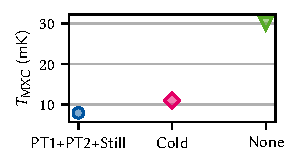
\includegraphics{img/pdf/setup/window_heating}
    \caption[\imgsource{img/py/setup/cooling_power.py}]{
        \Acrlong{mxc} temperature for different configurations of \gls{ar} coated windows (Thorlabs WW41050-B) inside the \gls{dr}.
    }
    \label{fig:setup:cooling:windows}
\end{marginfigure}

\begin{equation}\label{eq:setup:cooling:dr_power}
    P = \dot{Q} = \alpha T_{\mr{\acrshort{mxc}}}^2 + \beta
\end{equation}

\begin{marginfigure}
    \centering
    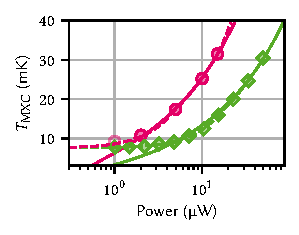
\includegraphics{img/pdf/setup/laser_heating}
    \caption[\imgsource{img/py/setup/cooling_power.py}]{
        \Acrlong{mxc} temperature as function of heater (magenta) and laser (green) power.
        Solid lines are fits to \cref{eq:setup:cooling:dr_power} including only the solid markers.
        Green dashed line is a quadratic smoothing spline fit to all laser data points.
        Magenta dashed line is the laser spline scaled to match the heater data with fitted factor $A=\qty{28}{\percent}$ corresponding to the fraction of laser power absorbed and non-radiatively emitted.
    }
    \label{fig:setup:cooling:laser}
\end{marginfigure}

\begin{marginfigure}
    \centering
    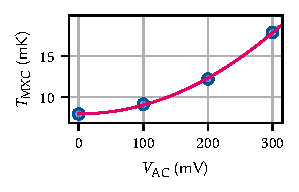
\includegraphics{img/pdf/setup/anc_readout_heating}
    \caption[\imgsource{img/py/setup/cooling_power.py}]{
        \Acrlong{mxc} temperature as function of nanopositioner AC readout voltage.
        Solid line is a fit to $T_{\mr{\acrshort{mxc}}} = a V_{\mr{AC}}^2 + b$.
        The secondary axis indicates the conversion from $T_{\mr{\acrshort{mxc}}}$ to power obtained in \cref{fig:setup:cooling:laser} which is approximately linear in this regime, leading to the expected $P\sim R\inverse V_{\mr{AC}}^2$ behavior.
        Fitting $P$ instead of $T_{\mr{\acrshort{mxc}}}$ results in $R=\qty{17.5}{\kilo\ohm}$.
        % TODO: check if V_AC is RMS or amplitude
    }
    \label{fig:setup:cooling:anc}
\end{marginfigure}

\section{Electron temperature}\label{sec:setup:cooling:etemp}
\begin{figure*}
    \centering
    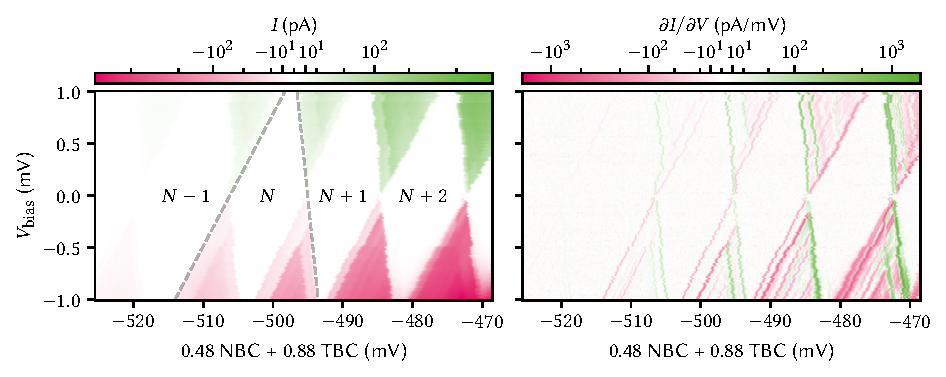
\includegraphics{img/pdf/setup/diamonds}
    \caption[\imgsource{img/py/setup/transport.py}]{}
    \label{fig:setup:cooling:etemp:diamonds}
\end{figure*}

\begin{marginfigure}
    \centering
    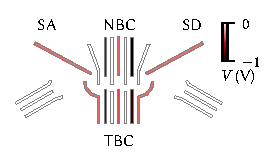
\includegraphics{img/pdf/setup/diamonds_gl}
    \caption[\imgsource{img/py/setup/transport.py}]{}
    \label{fig:setup:cooling:etemp:gl}
\end{marginfigure}

\begin{marginfigure}
    \centering
    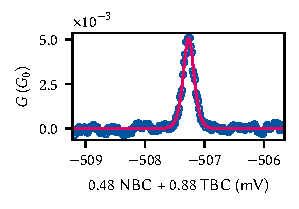
\includegraphics{img/pdf/setup/coulomb_resonance}
    \caption[\imgsource{img/py/setup/transport.py}]{}
    \label{fig:setup:cooling:etemp:resonance}
\end{marginfigure}
